\documentclass[tikz,border=3pt]{standalone}
\usepackage[T1]{fontenc}
\usepackage{mathptmx}
\usepackage{tikz,pgfplots}
\usetikzlibrary{arrows.meta,positioning,calc,fit,backgrounds,shapes.geometric}
\pgfplotsset{compat=1.18}
\definecolor{forest}{HTML}{346E57}
\definecolor{sage}{HTML}{E8EFEA}
\definecolor{clay}{HTML}{AC653F}
\definecolor{sand}{HTML}{F4EAE2}
\definecolor{ink}{HTML}{252525}
\definecolor{light}{HTML}{F5F5F3}
\definecolor{gridgray}{HTML}{D8DAD6}
\tikzset{box/.style={draw=ink!70,line width=.5pt,rectangle,rounded corners=1pt,fill=white,align=center,font=\fontsize{11}{12}\selectfont,inner sep=6pt}, flow/.style={-{Latex[length=2.4mm]},line width=.7pt,draw=ink!80}, data/.style={flow,densely dashed,draw=forest}, label/.style={font=\fontsize{10}{11}\selectfont,fill=white,inner sep=2pt,align=center}}
\hyphenpenalty=10000\exhyphenpenalty=10000\begin{document}
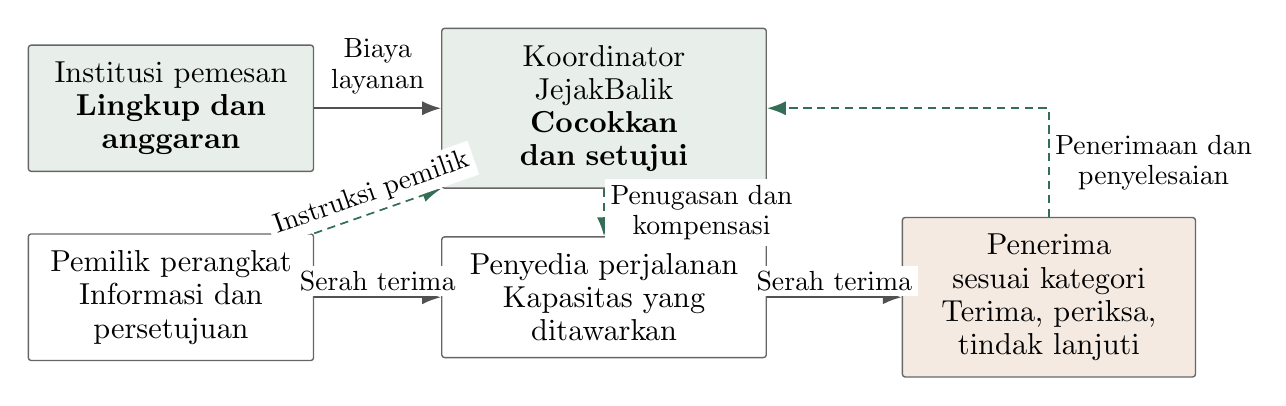
\begin{tikzpicture}[x=1cm,y=1cm]
\node[box,text width=3.2cm,fill=sage] (host) at (0,2.4) {Institusi pemesan\\\textbf{Lingkup dan anggaran}};
\node[box,text width=3.7cm,fill=sage] (coord) at (5.5,2.4) {Koordinator JejakBalik\\\textbf{Cocokkan dan setujui}};
\node[box,text width=3.2cm] (owner) at (0,0) {Pemilik perangkat\\Informasi dan persetujuan};
\node[box,text width=3.7cm] (carrier) at (5.5,0) {Penyedia perjalanan\\Kapasitas yang ditawarkan};
\node[box,text width=3.3cm,fill=sand] (receiver) at (11.15,0) {Penerima sesuai kategori\\Terima, periksa, tindak lanjuti};
\draw[flow] (host)--node[label,above=3pt]{Biaya\\layanan}(coord);

\draw[data] (coord)--node[label,right]{Penugasan dan\\kompensasi}(carrier);
\draw[flow] (owner)--node[label,above]{Serah terima}(carrier);
\draw[flow] (carrier)--node[label,above]{Serah terima}(receiver);
\draw[data] (receiver.north)|-node[label,near start,right]{Penerimaan dan\\penyelesaian}(coord.east);
\draw[data] (owner.north east)--node[label,above,sloped]{Instruksi pemilik}(coord.south west);
\end{tikzpicture}
\end{document}
